\documentclass[11pt, a4paper]{article}
\usepackage[T1]{fontenc}
\usepackage{geometry}
\usepackage{parskip}
\usepackage{microtype}
\usepackage{amsmath, amssymb, bm, esint}
\usepackage{graphicx}
\usepackage{physics, siunitx}
\usepackage{tikz}
\usepackage{hyperref}

% Begin package configuration
% --------------------------------------------- %
\sisetup{separate-uncertainty=true, exponent-product=\cdot, range-units=single}
\setcounter{secnumdepth}{2}
\hypersetup{colorlinks = true, allcolors=blue}
\graphicspath{{../figures/}}
\newcommand{\hmargin}{3.0cm}
\newcommand{\vmargin}{2.90cm}
\geometry{top=\vmargin, bottom=\vmargin, left=\hmargin, right=\hmargin}
% --------------------------------------------- %

% Begin minted setup
% --------------------------------------------- %
\usepackage{minted, tcolorbox}
\BeforeBeginEnvironment{minted}{\begin{tcolorbox}}
\AfterEndEnvironment{minted}{\end{tcolorbox}}
\setminted[python]{tabsize=2, breaklines}
% --------------------------------------------- %

% Begin bibliography setup
% --------------------------------------------- %
\usepackage{biblatex}
\addbibresource{sources.bib}
\nocite{*}  % Print uncited sources in bibliography
% --------------------------------------------- %

% Begin custom macros
% --------------------------------------------- %
\DeclareMathOperator{\sinc}{sinc}
\DeclareSIUnit{\decibell}{dB}
\newcommand{\diff}{\mathop{}\!\mathrm{d}}
\newcommand{\F}{\mathcal{F}}
\newcommand{\TODO}[1]{{\textbf{TODO:} {\color{red} #1}}}
% --------------------------------------------- %


\begin{document}

\thispagestyle{empty}
\begin{center}

    \definecolor{ul-red}{RGB}{220,29,39}
    \begin{figure}[htb!]
        \centering
        
\includegraphics[width=0.09\linewidth]{ul-logo}
    \end{figure}
    \LARGE{\textsc{University of Ljubljana}}\\
    \Large{\textsc{Faculty of {\color{ul-red} mathematics and physics}}}\\[1ex]
    \large{\textsc{Department of physics}}\\
    \vspace{5ex}
    \huge{Data Acquisition and Processing}\\
    \rule{0.9\textwidth}{0.2pt}\\[1ex] \LARGE{\textbf{Designing and implementing a near real-time bandpass Hilbert transformer}}
    \rule{0.9\textwidth}{0.2pt}

    \vspace{1ex}

    \begin{minipage}[t]{0.80\textwidth}
        \normalsize{\textsc{Author:}} \hfill \large{\textsc{Student ID}:}\\
    \large{Elijan Jakob Mastnak} \hfill \large{28181157}
    \end{minipage}

\end{center}

\vspace{5ex}
\begin{center}
    \textbf{Assignment}\\[2mm]
    \begin{minipage}[t]{0.80\textwidth}
        Use the window method with an appropriate window function to design an FIR band-pass Hilbert transform filter for use with signals sampled at $ f_{\mathrm{s}} = \SI{44100}{\hertz} $.
        The filter passband should span the frequency range from \SI{1000}{\hertz} to \SI{2000}{\hertz}; in the passband, the input and output signals should differ in phase by $ \pi/2 $ (as for a Hilbert transformer) and in amplitude by no more than one \SI{1}{\decibell}.
        For frequencies below \SI{500}{\hertz} and above \SI{2500}{\hertz}, the output signal's amplitude should be at least \SI{40}{\decibell} less than the input amplitude.
        Compute the FIR filter's coefficients, test the filter in an offline simulation, and finally ensure the filter works in real time.
        
    \end{minipage}

    \vfill
    \large{Ljubljana, September 2021}
\end{center}


\newpage
\tableofcontents
\newpage

\section{Computing the Filter's Impulse Response}

\subsection{Choosing a Window Function}

We select a window function from the requirement that the filter's stopband attenuation be less than \SI{-40}{\decibell}, which requires a filter with peak approximation error (PAE) less than \SI{-40}{\decibell} \cite{introdsp, proakis}.
% Compute passband and stopband ripple $ \delta_{\mathrm{p}} $ and $ \delta_{\mathrm{s}} $ according to
% \begin{equation*}
%     20 \log (1 + \delta_{\mathrm{p}}) \, \si{\decibell} = \SI{1}{\decibell} \implies \delta_{\mathrm{p}} = 10^{1/20} - 1 \approx 0.122
% \end{equation*}
% and
% \begin{equation*}
%     20 \log \delta_{\mathrm{s}} \, \si{\decibell} = - \SI{40}{\decibell} \implies \delta_{\mathrm{s}} = 10^{-2} = 0.01.
% \end{equation*}
% The smaller of these two is $ \delta_{\mathrm{s}} $, and the corresponding attenuation is \SI{-40}{\decibell}.
A number of common window functions are listed in Table \ref{tab:windows}; of these, the Hann, Hamming and Blackman windows all have a PAE less than \SI{-40}{\decibell}. In principle, any of these would work; I chose a Hann window to avoid over-designing the filter, i.e. to avoid increasing the filter's transition band width in exchange for larger-than-required stopband attenuation.

\begin{table}[htb!]
    \centering
    \begin{tabular}{|c|c|}
        \hline
        Frequency $ f $ & Attenuation \\
        \hline
        \hline
        $ f < \SI{500}{\hertz} $ & $ \abs{H} < \SI{-40}{\decibell} $ \\
        $ \SI{1000}{\hertz} < f < \SI{2000}{\hertz} $ & $ \abs{H} = \SI{0 \pm 1}{\decibell} $ \\
        $ f > \SI{2500}{\hertz} $ & $ \abs{H} < \SI{-40}{\decibell} $ \\
        \hline
    \end{tabular}
    \caption{The problem's filter specifications.}
    \label{tab:specs}
\end{table}

We estimate an appropriate number of window coefficients $ M $ by equating the known Hann window main lobe width of $ 8 \pi/M $ (from Table \ref{tab:windows}) to the filter's specified transition band width $ \Delta \omega $ in units of normalized frequency. First, referring to the specifications in Table \ref{tab:specs}, the filter's transition band width\footnote{In this problem the filter's upper and lower transition widths are both \SI{500}{\hertz}. If they were different, we would use the smaller (i.e. more restrictive) of the two.} is
\begin{equation*}
    \Delta f = \SI{1000}{\hertz} - \SI{500}{\hertz} = \SI{2500}{\hertz} - \SI{2000}{\hertz} = \SI{500}{\hertz}.
\end{equation*}%
The corresponding transition band width in units of normalized frequency is
\begin{equation*}
    \Delta \omega = 2\pi \frac{\Delta f}{f_{\mathrm{s}}} = 2\pi \frac{\SI{500}{\hertz}}{\SI{41000}{\hertz}} = \frac{\pi}{41}.
\end{equation*}
Using the just-computed transition band width $ \Delta \omega $, an appropriate number of filter coefficients $ M $ is
\begin{equation}
    \frac{8 \pi}{M} = \Delta \omega = \frac{\pi}{41} \implies M = 328. \label{eq:kernel_length}
\end{equation}
I implemented the actual filter with $ M + 1 = 329 $ coefficients, since an odd-length impulse response is more conducive to implementing a bandpass filter.\footnote{Specifically, implementing a Hilbert transform produces an antisymmetric impulse response, and the frequency response of filter with odd-length, antisymmetric impulse response has zeros at $ f = \SI{0}{\hertz} $ (DC) and at $ f = f_{\mathrm{s}}/2 $ (the Nyquist rate) \cite{introdsp}. This zero configuration is well-suited to a bandpass filter.}

\begin{table}[htb!]
        \centering
        \begin{tabular}{|c|c|c|}
            \hline
            Window Function & MLW & PAE $ [\si{\decibell}] $\\
            \hline
            \hline {\rule{0pt}{2.6ex}} \hspace{-7pt}
            Rectangular & $ \frac{4\pi}{M + 1} $ & $ -21 $\\[0.5ex]
            Hann & $ \frac{8\pi}{M} $ & $ -44 $\\[0.5ex]
            Hamming & $ \frac{8\pi}{M} $ & $ -53 $\\[0.5ex]
            Blackman & $ \frac{12 \pi}{M} $ & $ -74 $\\[0.3ex]
            \hline
        \end{tabular}     
        \caption{Approximate main lobe width (MLW), in units of normalized frequency, and peak approximation error (PAE) of common window functions. $ M $ denotes the number of coefficients used to implement the window (and filter). Taken from \cite{proakis}.}
        \label{tab:windows}
\end{table}

\subsection{Computing Filter's Impulse Response}
Below is an outline of the process used to compute the filter's impulse response:
\begin{enumerate}

    \item Compute the impulse response $ h_{\mathrm{lp}} $ of an ideal \textit{lowpass} filter.

    \item Write the impulse response $ h_{\mathrm{pb}} $ of an ideal \textit{bandpass} filter as the difference of two lowpass impulse responses.
    
    \item Separately compute the impulse response $ h_{\mathrm{H}} $ of an ideal Hilbert transformer.

    \item Write the complete filter's ideal impulse response as the convolution $ h_{\mathrm{bp}} * h_{\mathrm{H}} $.

    \item Truncate and window the ideal impulse response to get the finite-length impulse response actually implemented in software.

\end{enumerate}

\subsubsection{Ideal Lowpass Impulse Response}
The frequency response of an ideal lowpass filter with continuous-time cutoff frequency $ \Omega_{\mathrm{c}} $ is the rectangular function
\begin{equation*}
    H_{\mathrm{lp}}(i \Omega) =
    \begin{cases}
        1 & -\Omega_{\mathrm{c}} < \Omega < \Omega_{\mathrm{c}}\\
        0 & \text{otherwise}.
    \end{cases}
\end{equation*}
The corresponding continuous-time impulse response is
\begin{align*}
    h_{\mathrm{lp}}(t) & = \frac{1}{2\pi} \int_{-\infty}^{\infty} H(i \Omega) e^{i \Omega t} \diff \Omega = \frac{1}{2\pi} \int_{-\Omega_{\mathrm{c}}}^{\Omega_{\mathrm{c}}} e^{i \Omega t} \diff \Omega = \frac{1}{2\pi i t} \Big[ e^{i \Omega t} \Big]_{-\Omega_{\mathrm{c}}}^{\Omega_{\mathrm{c}}}\\
    & = \frac{1}{2\pi i t} \big( e^{i \Omega_{\mathrm{c}} t} - e^{-i \Omega_{\mathrm{c}} t} \big) = \frac{\sin \Omega_{\mathrm{c}} t}{\pi t}\\[0.3ex]
    & = \frac{\Omega_{\mathrm{c}}}{\pi} \sinc (\Omega_{\mathrm{c}} t).
\end{align*}
We convert the continuous-time impulse response to discrete time (assuming sample rate $ f_{\mathrm{s}} = 1/T $) by changing $ t \to n T $ and including an amplitude scaling factor $ T = 1/f_{\mathrm{s}} $, i.e.
\begin{equation}
    h_{\mathrm{lp}}[n] = T \cdot \frac{\Omega_{\mathrm{c}}}{\pi} \sinc [\Omega_{\mathrm{c}} n T] = \frac{2 f_{\mathrm{c}}}{f_{\mathrm{s}}} \sinc \left[ \frac{2\pi f_{\mathrm{c}}}{f_{\mathrm{s}}} n \right]. \label{eq:hlp}
\end{equation}

\subsubsection{Ideal Bandpass Impulse Response}
The impulse response of an ideal \textit{bandpass} filter with high and low passband frequencies $ f_{\mathrm{high}} $ and $ f_{\mathrm{low}} $ may be constructed as the difference of two lowpass filters with cutoff frequencies $ f_{\mathrm{high}} $ and $ f_{\mathrm{low}} $, respectively \cite{ponikvar}, i.e.
\begin{align*}
    h_{\mathrm{bp}}[n] & = h_{\mathrm{lp}}[n; f_{\mathrm{high}}] - h_{\mathrm{lp}}[n; f_{\mathrm{low}}]\\[0.3ex]
    & = \frac{2 f_{\mathrm{high}}}{f_{\mathrm{s}}} \sinc \left[ \frac{2\pi f_{\mathrm{high}}}{f_{\mathrm{s}}}n \right] - \frac{2 f_{\mathrm{low}}}{f_{\mathrm{s}}} \sinc \left[ \frac{2\pi f_{\mathrm{low}}}{f_{\mathrm{s}}} n \right].
\end{align*}
This impulse response has a removable discontinuity at $ n = 0 $ which must be treated separately in a computer implementation. Using the limit $ \lim_{x \to 0} \sinc x = 1 $, this is
\begin{equation*}
    h_{\mathrm{bp}}[0] = \frac{2}{f_{\mathrm{s}}}(f_{\mathrm{high}} - f_{\mathrm{low}}).
\end{equation*}

\subsubsection{Ideal Hilbert Transformer Impulse Response}
The frequency response of an Hilbert transformer for frequencies in the range $ (-\Omega_{0}, \Omega_{0}) $ is
\begin{equation*}
    H_{\mathrm{H}} (i\Omega) = 
    \begin{cases}
        e^{- i \frac{\pi}{2}} & -\Omega_{0} < \Omega < 0\\
        e^{+ i \frac{\pi}{2}} & 0 < \Omega < \Omega_{0} \\
        0 & \text{otherwise}.
    \end{cases}
\end{equation*}
The corresponding continuous-time impulse response is
\begin{align*}
    h_{\mathrm{H}}(t) & = \frac{1}{2\pi} \int_{-\infty}^{\infty} H(i \Omega) e^{i \Omega t} \diff \Omega = \frac{1}{2\pi} \int_{-\Omega_{0}}^{0} e^{-i \frac{\pi}{2}} e^{i \Omega t} \diff \Omega + \frac{1}{2\pi} \int_{0}^{\Omega_{0}} e^{+i \frac{\pi}{2}} e^{i \Omega t} \diff \Omega\\
    & = \frac{1}{2\pi i t} \left[ e^{+i (\Omega_{0} t + \pi/2)} - e^{-i (\Omega_{0} t + \pi/2)} \right] - \frac{1}{2\pi i t} \left( e^{+i \frac{\pi}{2}} - e^{-i \frac{\pi}{2}} \right)\\
    & = \frac{1}{\pi t} \sin(\Omega_{0} t + \pi/2) - \frac{\sin(\pi/2)}{\pi t}\\
    & = \frac{1}{\pi t} \big[ \cos (\Omega_{0} t) - 1 \big].
\end{align*}
As in Equation \ref{eq:hlp} for the lowpass filter, we convert to discrete time by changing $ t \to n T $ and including an amplitude scaling factor $ T = 1/f_{\mathrm{s}} $, i.e.
\begin{equation*}
    h_{\mathrm{H}}[n] = \frac{T}{\pi n T} \big( \cos [\Omega_{0} n T] - 1 \big) = \frac{1}{\pi n} \left( \cos \left[ \frac{2\pi f_{0}}{f_{\mathrm{s}}} n\right] - 1 \right).
\end{equation*}
If the Hilbert transformer is to apply to the entire discrete frequency domain, i.e if $ f_{0} = f_{\mathrm{s}}/2 $, the impulse response simplifies considerably to
\begin{align*}
    h_{\mathrm{H}}[n] & = \frac{1}{\pi n} \left( \cos \left[ \frac{2\pi f_{\mathrm{s}}}{2 f_{\mathrm{s}}} n\right] - 1 \right) = \frac{1}{\pi n} \big( \cos [\pi n] - 1 \big)\\
& = \frac{1}{\pi n} \big[ (-1)^{n} - 1 \big].
\end{align*}
However, this problem's specifications require the filter shift phase by $ \pi/2 $ only in the passband, so I choose a Hilbert transform cutoff frequency $ f_{0} = \SI{3000}{\hertz} $ instead of using the Nyquist rate $ f_{0} = f_{\mathrm{s}}/2 = \SI{22500}{\hertz} $.

\subsubsection{Complete Ideal Impulse Response}
Convolution is commutative and associative, which simplifies the practical implementation of the filter's impulse response. Namely, processing an input signal, say $ x $, with a bandpass filter with impulse response $ h_{\mathrm{bp}} $ and then passing the filtered signal, say $ x_{\mathrm{f}} $, through a Hilbert transformer with impulse response $ h_{\mathrm{H}} $ is equivalent to passing the input $ x $ through a single system whose impulse response is the convolution of $ h_{\mathrm{bp}} $ and $ h_{\mathrm{H}} $. This is shown symbolically in Equation \ref{eq:conv-assoc} and graphically in Figure \ref{fig:conv-assoc}.

\begin{equation}
    y = h_{\mathrm{H}} * x_{\mathrm{f}} = h_{\mathrm{H}} * ( h_{\mathrm{bp}} * x ) = (h_{\mathrm{H}} * h_{\mathrm{bp}}) * x \equiv h_{\mathrm{total}} * x. \label{eq:conv-assoc}
\end{equation}
\begin{figure}[htb!]
    \centering
    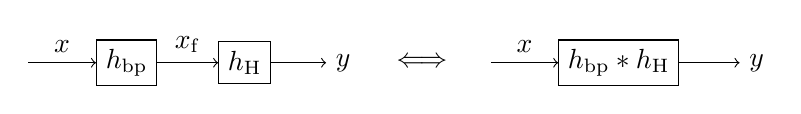
\begin{tikzpicture}
            \pgfmathsetmacro{\dx}{1.25}
            \path (0,0) node[rectangle, draw] (bp) at ++(\dx, 0) {$ h_{\mathrm{bp}} $}; % bandpass filter box
            \path (bp) node[rectangle, draw] (H) at ++(1.2*\dx, 0) {$ h_{\mathrm{H}} $};  % hilbert transform
            \path (H) node (y) at ++(\dx, 0) {$ y $}; % ouput z

            % arrows
            \draw[->] (0, 0) -- (bp) node [midway, above] {$ x $};
            \draw[->] (bp) -- (H) node [midway, above] {$ x_{\mathrm{f}} $};
            \draw[->] (H) -- (y);

            \node at (4*\dx, 0) {$ \iff $};  % iff equivalence arrow
            % one-stage convolved version
            \begin{scope}[shift={(5*\dx, 0)}]
                \path (0,0) node[rectangle, draw] (h) at ++(\dx, 0) {$ h_{\mathrm{bp}} * h_{\mathrm{H}} $}; % convolved filter
                \path (h) node (y) at ++(1.4*\dx, 0) {$ y $}; % ouput y

            % arrows
                \draw[->] (-0.3*\dx, 0) -- (h) node [midway, above] {$ x $};
                \draw[->] (h) -- (y);
            \end{scope}
        \end{tikzpicture}    
        \caption{Convolution's associativity simplifies the filter implementation: the left and right systems produce identical outputs, but if $ h_{\mathrm{bp}}*h_{\mathrm{H}} $ is computed beforehand, implementing the right version in real-time requires half as many convolutions. C.f. Equation \ref{eq:conv-assoc}.}
        \label{fig:conv-assoc}
\end{figure}

The complete filter's ideal impulse response is thus
\begin{equation*}
    h_{\mathrm{ideal}} = h_{\mathrm{bp}} * h_{\mathrm{H}}.
\end{equation*}

\subsubsection{Windowed Impulse Response}

The discrete Hann window function for a filter with $ M + 1 $ coefficients is
\begin{equation*}%
    w[n] = 
    \begin{cases}
        \frac{1}{2} \left( 1 + \cos \left[ \frac{2\pi n}{M} \right] \right) & n = - \frac{M}{2}, \ldots, \frac{M}{2}\\
        0 & \text{otherwise}.
    \end{cases}
\end{equation*}
The corresponding causal window, with center shifted to $ n = M/2 $, is
\begin{equation*}
    w_{\mathrm{causal}}[n] = w[n - M/2] = 
    \begin{cases}
        \frac{1}{2} \left( 1 - \cos \left[ \frac{2\pi n}{M} \right] \right) & n = 0, \ldots, M\\
        0 & \text{otherwise}.
    \end{cases}
\end{equation*}
The windowed impulse response is
\begin{equation*}
    h[n] = h_{\mathrm{ideal}}[n - M/2] w_{\mathrm{causal}}[n].
\end{equation*}
The code used to compute $ h[n] $ appears in the \texttt{get\_h} function in the file \texttt{bandpass.py}.\footnote{I initially thought to put the full code in an appendix, but doing so added $ \sim 15 $ additional pages to the report and wasn't appreciably easier to read than the source files themselves, which I have left separate.}

\begin{figure}[htb!]
	\centering
	\includegraphics[width=\linewidth]{h-all}
    \vspace{-3ex}
	\caption{Windowed impulse responses of the bandpass and Hilbert transformer stages (left and center), together with their convolution (right).}
	\label{fig:h-all}
\end{figure}

\subsection{Visualizing the Filter's Impulse and Frequency Responses}
Figure \ref{fig:h-all} shows the windowed impulse responses of the bandpass stage, the Hilbert transformer stage, and the convolution of the two stages. Figure \ref{fig:H-abs} shows the frequency response of the convolved bandpass-Hilbert system both with and without windowing. As expected theoretically, windowing the impulse response produces a far smoother frequency response and better stopband attenuation at the expense of a wider transition band. Figure \ref{fig:H-abs-close} attempts to demonstrate that the filter meets the specifications in Table \ref{tab:specs}. Finally, Figure \ref{fig:H-angle} shows the filter's phase response---the discontinuity in phase angle at $ f = \SI{0}{\hertz} $ and $ \theta \approx - \ang{45} $ shows the phase-shifting effect of the Hilbert transformer.

\newpage

% hack to fit three figures on one page
\newgeometry{top=2.5cm, bottom=2cm, left=\hmargin, right=\hmargin, footskip=-20pt}

\begin{figure}[htb!]
	\centering
	\includegraphics[width=\linewidth]{H-abs}
    \vspace{-3.5ex}
	\caption{Windowed and un-windowed frequency responses.}
	\label{fig:H-abs}
\end{figure}

\begin{figure}[htb!]
	\centering
	\includegraphics[width=0.85\linewidth]{H-abs-close}
    \vspace{-2ex}
	\caption{The filter's frequency response in the transition and passband regions. The curve must not touch the shaded grey areas to meet the filter specifications in Table \ref{tab:specs}.}
	\label{fig:H-abs-close}
\end{figure}

\begin{figure}[htb!]
	\centering
	\includegraphics[width=0.85\linewidth]{H-angle}
    \vspace{-2ex}
	\caption{The filter's phase response. The phase is linear in the passband, while the discontinuity at $ f = \SI{0}{\hertz} $ corresponds to the Hilbert transformer phase shift.}
	\label{fig:H-angle}
\end{figure}

\clearpage
\restoregeometry

\section{Implementing Real-time Filtering}
The hardware and software used to implement the filter is summarized below:
\begin{itemize}

    \item Computer: 13-inch, 2012 MacBook Pro laptop with a \SI{2.5}{\giga \hertz} Intel Core i5 processor running macOS 10.14.6. Audio was captured using the laptop's built-in \SI{44100}{\hertz}, 2-channel microphone, but only one channel was used as filter input.

    \item I used version 19 of the \texttt{PortAudio} library \cite{portaudio}, which is an audio I/O library written in C, to capture the audio input stream from the computer's microphone.

    \item I wrote the filter program in Python and used the \texttt{PyAudio} library \cite{pyaudio} to provide Python bindings for the C code in \texttt{PortAudio}.
    I used the \texttt{NumPy} library \cite{numpy} for efficient implementation of the fast Fourier transform, convolution, and common mathematical functions.

\end{itemize}
Source code and a video demonstration of the filter's real-time functionality can be found in an online repository, and a summary of how the real-time filtering works follows below.
% \TODO{reference}.


Audio data is captured from the microphone using \texttt{PortAudio} with an input stream with the specifications shown in Table \ref{tab:stream}. The number of frames per buffer is chosen so that the fast Fourier transform used to convolve the impulse response with the audio buffer has 4096 elements (i.e. a power of two, which is a general best practice for FFT algorithms). The initialization of the audio stream is shown in Listing \ref{code:stream}.

\begin{table}[htb!]
    \centering
    \begin{tabular}{|c|c|}
        \hline
        Parameter & Value\\
        \hline
        \hline
        Sample rate & \SI{44100}{\hertz}\\
        Format & 32-bit floating point\\
        Channels & 1\\
        Frames per buffer & $ 4096 - \texttt{len(h)} + 1 $\\
        \hline
    \end{tabular}
    \caption{Audio stream parameteters. \texttt{len(h)} is the length of the filter's impulse response.}
    \label{tab:stream}
\end{table}

\begin{listing}[htb!]
\begin{minted}{python}
import numpy as np
import pyaudio
h = get_h()  # load impulse response from separate function
CHUNK = 4096 - len(h) + 1  # frames per buffer
pa = pyaudio.PyAudio()
stream = pa.open(format=pyaudio.paFloat32,  # 32-bit floating point
        channels=1,  # use only single-channel audio
        rate=44100,  # sample rate [Hz]
        input=True,  # use this stream as an input stream
        frames_per_buffer=CHUNK)
stream.start_stream()
\end{minted}
    \vspace{-1ex}
    \caption{Source code for initializing the audio stream.}
    \label{code:stream}
\end{listing}

Data is read from the audio stream as a hexadecimal Python byte string, which is then converted to an array of 32-bit floating point numbers with \texttt{NumPy}'s \texttt{frombuffer} function. For orientation, a representative audio stream output buffer is shown in Listing \ref{code:output}.
The real-time filtering process works by convolving each buffer of audio data with the filter's impulse response using the overlap-add method \cite{convolution}.
The code implementing the overlap-add method, with explanatory comments, appears in Listing \ref{code:filter}.

One specific feature of the code in Listing~\ref{code:filter} deserves special comment.
First, here is the context: the real-time filtering program listens for input audio data and displays a continuously-updated plot of both the unfiltered input audio waveform and its bandpass-filtered and Hilbert-transformed version.
The input and filtered signal are intentionally shown together on the same time-domain plot to verify the filter's phase-shifting property, as in e.g. Figure~\ref{fig:phase}.
Resultantly, it is important that the unfiltered input signal and its filtered version correctly align in the time domain.
FIR filtering inherently introduces a time delay to the filtered signal equal to the length $ M $ of the FIR filter kernel.
To compensate for this delay, the code in Listing~\ref{code:filter} creates a delayed copy of the unfiltered input signal by convolving the raw input signal with a unit impulse centered at $ M / 2 $.
This delayed version of the input signal and its FIR-filtered analog are then correctly aligned in the time domain.

\begin{listing}
\begin{minted}{python}
>>> buffer = stream.read(10)  # read 10 frames
b'\x00\x82\x00\xe0\x9a\x00\x8c\xb0\x00<\x97\x00\xa0\x9c\x00\xfc\x92\x00 \xc4\xbb\x00\x00\xf8\xa3\x00\x10'
>>> buffer_float32 = np.frombuffer(data, dtype=np.float32)
[0.2548523  0.30249023 0.34481812 0.29537964 0.3059082  0.28707886  0.36672974 0.23553467 0.32025146 0.22174072]
\end{minted}   
    \vspace{-1ex}
    \caption{Representative audio stream output as a byte string and corresponding 32-bit floating point array (which has been rounded for conciseness).}
    \label{code:output}
\end{listing}

\begin{listing}
\begin{minted}{python}
import numpy as np

# Load filter's impulse response from separate function
h = get_impulse_response()
M = len(h)  # length of impulse response

# Create a delay-by-M kernel to compensate FIR-induced delay 
h_delay_by_M = np.zeros(M, dtype=np.float32)
h_delay_by_M[int((M - 1)/2)] = 1.0

# Declare global variable to store last `M` points of previous
# iteration's convolution of filter kernel and audio buffer
filter_conv_prev = np.zeros(M - 1)  # preallocate with zeros

# Global variable to store last `M` points of previous
# iteration's convolution of delay-by-M kernel and audio buffer
conv_delayed_prev = np.zeros(M - 1)

def get_filtered_audio_buffer(buffer_in):
    """
    Applies the Hilbert transform filter to the inputted audio buffer
    `buffer_in`. Returns filtered output `buffer_out` and delayed
    copy of `buffer_in` aligned in time with `buffer_out`.
    """
    L = len(buffer_in)
    # Convolve kernel `h` and `buffer_in` and store first `L` points
    filter_conv = np.convolve(h, buffer_in)
    buffer_out = filter_conv[:L]

    # Append last `M-1` elements of previous iteration's convolution
    # to first `M-1` elements of current convolution
    buffer_out[:M - 1] += filter_conv_prev

    # Save last `M-1` elements of this iteration's convolution for
    # use in the next iteration
    filter_conv_prev = filter_conv[-(M - 1):]

    # Create delayed copy of `buffer_in` aligning with `buffer_out`
    delay_conv = np.convolve(h_delay_by_M, buffer_in)
    buffer_in_delayed = delay_conv[:L]
    buffer_in_delayed[:M - 1] += delay_conv_prev
    delay_conv_prev = delay_conv[-(M - 1):]

    return buffer_in_delayed, buffer_out
\end{minted}
    \vspace{-1ex}
    \caption{The function \texttt{get\_filtered\_buffer} implements the overlap-add method used for real-time filtering. Complete code for real-time filtering is in the \texttt{realtime.py} file in the project's source code repository \TODO{reference}.}
    \label{code:filter}
\end{listing}

\section{Representative Filtered Signals}
The following few figures were generated offline, all with sample rate $ f_{\mathrm{s}} = \SI{44100}{\hertz} $, and are meant to demonstrate the filter's desired phase shift and bandpass properties in an offline scenario.
A demonstration of the filter's real-time functionality may be seen in an online demonstration video \TODO{reference}.

\begin{figure}[htb!]
	\centering
	\includegraphics[width=0.85\linewidth]{test-time-shift}
    \vspace{-3ex}
	\caption{Demonstration of the filter's phase-shifting property with a \SI{1500}{\hertz} sinusoid. 
    The dotted curve with blue circular markers is a copy of the input signal shifted by $ \pi/2 $, which the filtered output (in maroon-red) aligns with nicely, as it must to satisfy the phase-shifting property of a Hilbert transformer.}
	\label{fig:phase}
\end{figure}

\begin{figure}[htb!]
	\centering
	\includegraphics[width=\linewidth]{test-square}
    \vspace{-5ex}
	\caption{The filter's time domain and frequency domain output in response to a 10-term Fourier series approximation of a square wave with fundamental frequency $ f_{0} = \SI{1200}{\hertz} $. All higher harmonics are filtered out, leaving only the \SI{1200}{\hertz} sinusoidal carrier wave in the filtered output. Note also the $ \ang{90} $ phase shift between the input and output signals.}
	\label{fig:square}
\end{figure}

\begin{figure}[htb!]
	\centering
	\includegraphics[width=\linewidth]{test-bandpass}
    \vspace{-5ex}
	\caption{The filter's time domain and frequency domain responses to a signal containing sinusoidal terms with frequencies $ (300, 500, 1500, 2500, 2700) \, \si{\hertz} $, all of equal amplitude. Only the \SI{1500}{\hertz} component in the passband is passed through the filter.}
	\label{fig:bandpass}
\end{figure}

\clearpage
\printbibliography

\end{document}
